This chapter will present the results of calculations using each of the decusping methods described in the previous chapter.  First, results for the polynomial and subplane collision probabilities methods will be presented.  The subplane collision probabilities results are presented as two sets of data: one with just subplane (axial correction only) and one with both subplane and CP (axial and radial), allowing the difference in magnitude between the axial and radial effects of the rod to be determined.  These methods were tested using the VERA Progression Problems \cite{VERAProgressionProblems}, a series of benchmark problems based on the Watts Bar Unit 1 \hl{cite} reactor that provide realistic test cases for the 2D/1D methods.  The control rods in these models were moved to various locations that stress the mesh typically used by MPACT to solve these problems, allowing the benefit of the decusping techniques to be clearly seen.  For some of these problems, detailed 3D power distributions were generated using the Monte Carlo code KENO-VI \hl{cite}, allowing for comparisons of the decusping methods with both refined MPACT meshes and Monte Carlo reference solutions.

In the second half of the chapter, results for the subray method of characteristics will be presented.  The first set of results come from the 1D prototype code discussed in section \hl{number}.  This code provided a quick implementation to show that it was worth pursuing the method in a full-scale transport code.  After this, results from MPACT's implementation of subray MOC will be presented for both 2D and 3D problems.  These results will be compared to refined mesh solutions in MPACT as well as the polynomial and subplane collision probabilities solutions to determine the relative accuracy of each of these methods.  All subray MOC results will use the C5G7 benchmark problems \cite{EELewisC5G72003,EELewisC5G7extended2005}.  Because these problems have specified macroscopic cross sections, some of the complexities of cross section processing and shielding calculations for subray MOC can be deferred to later research while still examining the accuracy and performance of subray MOC compared with other solutions to the rod cusping problem.

\section{VERA Problem 4}

\begin{figure}[h]\label{f:p4layout}
    \centering
    \subfigure{\label{f:p4radial}
        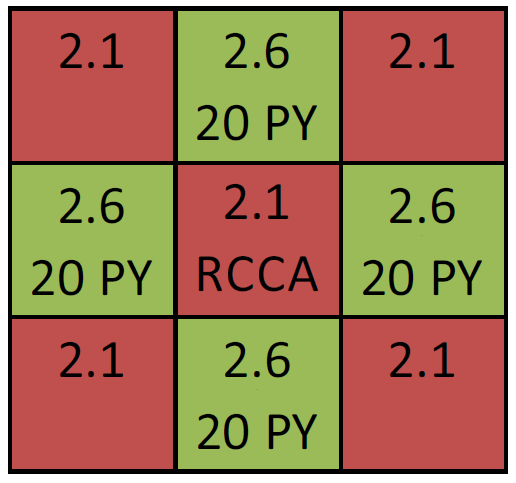
\includegraphics[width=0.4\textwidth]{p4a_layout.png}
    }
    ~
    \subfigure{\label{f:p4axial}
        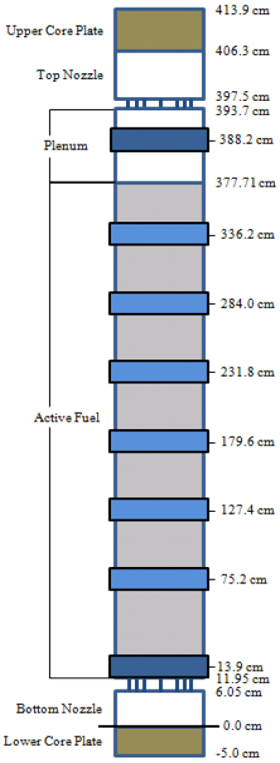
\includegraphics[width=0.3\textwidth]{wb_3d_assembly.png}
    }
    \caption{VERA Problem 4 radial (left) and axial (right) layouts}\label{f:p4}
\end{figure}

VERA Progression Problem 4 is composed of a 3x3 set of Westinghouse 17$\times$17 fuel assemblies with an active fuel height of 365.76 cm and a control bank in the center assembly.  The radial layout of the problem is shown in Figure \ref{f:p4radial}, and the axial layout of each assembly is shown in Figure \ref{f:p4axial}.  The control rods were placed at an axial elevation of 257.9 cm above the core plate, about one third inserted into the core.  The rod in the original problem specification is made of AIC with a B$_4$C follower and a stainless steel tip.  First, results will be presented which use several difference uniform rods to simplify the analysis, then results will be presented with the heterogeneous rod.  Lastly, a differential rod worth developed with the heterogeneous rod is shown with comparisons to KENO-VI reference solutions at regular intervals along the curve.

\subsection{Homogeneous Control Rods}

For the reference solution, 58 MOC planes were used with 49 of them in the active fuel region.  It was also ensured that the end of the control rods were exactly aligned with one of the MOC plane boundaries.  The cases with decusping methods used the same mesh, but with the 2 MOC planes around the tip of the control rod merged into a single plane to introduce cusping effects.  The accuracy and convergence data for these cases are shown in Table \ref{t:homoDecusp}.

\begin{table}[ht]
    \centering
    \caption{Comparison of Rod Decusping Methods in MPACT for VERA Progression 
        Problem 4 for Homogeneous Control Rods}
    \resizebox{\textwidth}{!}{\begin{tabular}{l l S[table-format=3.1,table-number-alignment=left] 
            S[table-format=1.3,table-number-alignment=left] 
            S[table-format=2.3,table-number-alignment=left] 
            S[table-format=2.1,table-number-alignment=left] l}\toprule
        \multirow{2}{*}{Rod Material} & \multirow{2}{*}{{Case}} & {k$_{eff}$} & 
        \multicolumn{2}{l}{{Pin Power 
                Differences}} & \multirow{2}{*}{{2D/1D Iterations}} & {Runtime}\\
        & & {Difference (pcm)} & {RMS} & {Max} &  & {(Core-Hours)} \\\midrule
        \multirow{5}{*}{AIC}      & Reference        & {--}  &    {--} &     {--} & 15 & 19.6 \\
                                  & No treatment     & -29.5 & 1.531\% & 11.839\% & 12 & 14.7 \\
                                  & Polynomial       &  -0.3 & 0.444\% &  4.081\% & 12 & 14.3 \\
                                  & Subplane         & -11.5 & 0.726\% &  8.209\% & 12 & 14.2 \\
                                  & Subplane + CP    &  -5.6 & 0.368\% &  4.248\% & 12 & 15.3\\\midrule
        \multirow{5}{*}{B$_4$C}   & Reference        & {--}  &    {--} &     {--} & 15 & 16.9 \\
                                  & No treatment     & 112.0 & 6.978\% & 69.372\% & 12 & 12.7 \\
                                  & Polynomial       & 112.6 & 6.886\% & 66.731\% & 12 & 12.1 \\
                                  & Subplane         & -17.9 & 1.142\% & 11.357\% & 13 & 15.2 \\
                                  & Subplane + 1D-CP & -11.0 & 0.687\% &  6.367\% & 12 & 13.4 \\\midrule
        \multirow{5}{*}{Tungsten} & Reference        & {--}  & {--}   &      {--} & 15 & 23.5 \\
                                  & No treatment     &  -8.4 & 0.370\% &  3.374\% & 12 & 15.5 \\
                                  & Polynomial       &  -4.4 & 0.239\% &  2.720\% & 12 & 14.5 \\
                                  & Subplane         &   1.6 & 0.069\% &  0.598\% & 12 & 13.9 \\
                                  & Subplane + CP    &  -0.9 & 0.055\% &  0.941\% & 12 & 15.6 \\\bottomrule
    \end{tabular}}
    \label{t:homoDecusp}
\end{table}

\hl{The ``No Treatment'' case shows the magnitude of the cusping effects for this problem.  The k$_{eff}$ difference is 30 pcm, which is not too alarming.  However, the RMS and maximum power differences are almost 4\% and over 20\%, respectively, which is an unacceptable level of error.  The polynomial decusping significantly reduces these errors to about 1\% and 6.5\% respectively.  This is much better, but still quite high.  The sub-plane decusping with no radial treatment performs similarly to the polynomial decusping, but slightly worse.  Because the polynomials were generated using this problem, it is expected that they would perform well.  Thus, the fact that the sub-plane decusping is comparable indicates that it is capturing the axial shape well.  Finally, the CP-based decusping gives the best results, with an RMS of about 0.5\% and a maximum error just under 5\%.  The maximum error is still larger than what is typically desired from the 2D/1D method, but is better than the old decusping treatment and far better than no treatment at all.}

\hl{As far as runtime is convergence and runtime is concerned, all cases took the same number of 2D/1D iterations.  The sub-plane--based decusping methods incurred a few more CMFD iterations, but this did not have a significant impact on runtime.  The difference in runtime between the reference and no treatment cases is due to the decomposition of the problem.  Both cases use the same sub-plane CMFD mesh (with homogeneous cross-sections in each plane).  However, the reference case was run with two MOC planes instead of one.  This also means that an extra core was used in the calculation.  Because of this, the time required for the transport calculations was the same, but the CMFD solve was slower for the no treatment case since a single core was solving a portion of the CMFD system handled by two cores in the reference calculation.  Thus, the runtime increase is due only to the parallel partitioning, not the methods themselves.  This is important, because the runtimes of the decusping cases were all about the same as the no treatment case.  This implies that the runtime penalty due to the decusping solvers is negligible.  Some work simply needs to be done to improve the parallel balance when using the sub-plane scheme.}

\subsection{Heterogeneous Control Rod}

Next, the same set of results can be shown again, but with the heterogeneous rod.  The same 58-plane reference mesh was used for these results.  However, the decusping cases have only 55 planes instead of 57.  This is needed to account for all three material interfaces in the heterogeneous rod: B$_4$C/AIC, AIC/SS, and SS/moderator.  The decusping methods are applied at all three of these locations simultaneously.  The results are shown in Table \ref{t:hetDecusp}.

\begin{table}[ht]
    \centering
    \caption{Comparison of Rod Decusping Methods in MPACT for VERA Progression 
        Problem 4 for Heterogeneous Control Rod}
    \begin{tabular}{l S[table-format=2.1,table-number-alignment=left] l 
            S[table-format=2.3,table-number-alignment=left] l l}\toprule
        \multirow{2}{*}{Case} & {k$_{eff}$} & \multicolumn{2}{l}{{Pin Power 
                Differences}} & \multirow{2}{*}{{2D/1D Iterations}} & {Runtime}\\
        & {Difference (pcm)} & {RMS} & {Max} &  & {(Core-Hours)} \\\midrule
        Reference        &  {--} &    {--} &     {--} & 15 & 16.6 \\
        No treatment     & -45.9 & 2.427\% & 20.450\% & 12 & 13.8 \\
        Polynomial       &  -2.5 & 0.457\% &  5.067\% & 12 & 13.0 \\
        Subplane         & -17.3 & 1.101\% & 11.771\% & 13 & 14.9 \\
        Subplane + CP    &  -5.5 & 0.415\% &  3.866\% & 12 & 14.7 \\\bottomrule
    \end{tabular}
    \label{t:hetDecusp}
\end{table}

\hl{Say some things about this}

\subsection{Differential Rod Worth Curve}

\begin{figure}[h]
    \centering
    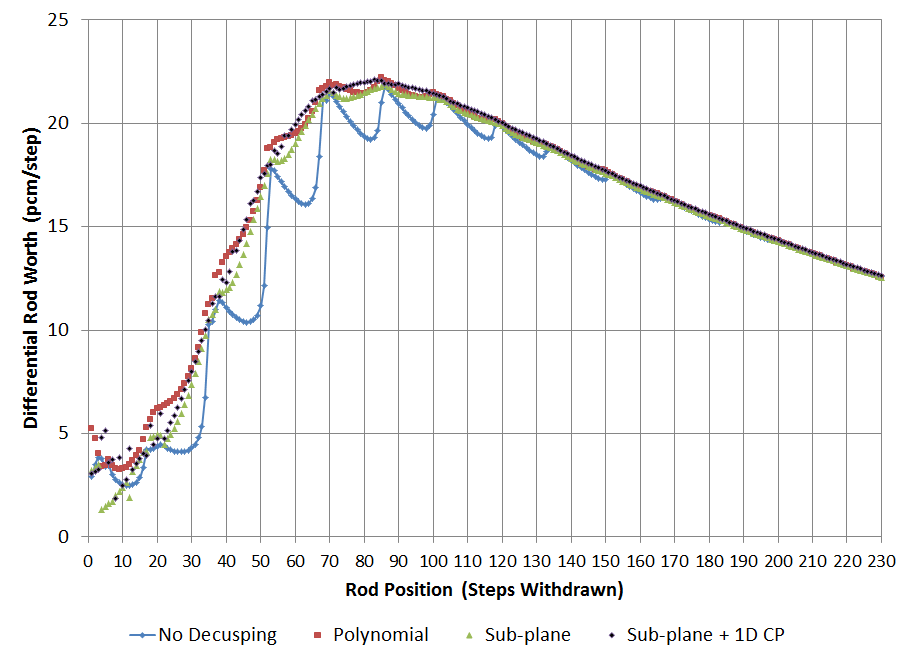
\includegraphics[width=\textwidth]{../../figs/differentialRodworth.png}
    \caption{Differential rod worth curves for MPACT decusping 
        techniques.}\label{f:rodworth}
\end{figure}

To show the effectiveness of each decusping technique as the rod moves upward through the reactor, a differential rod worth curve was developed for each method.  This curve is shown in Figure \ref{f:rodworth}.  \hl{Say some things}

\subsection{KENO-VI Comparisons}

\begin{table}[h]
    \centering
    \caption{Average Differences between MPACT and KENO-VI for VERA Problem 
        4}\label{t:keno}
    \sisetup{separate-uncertainty=true,table-text-alignment=left,table-number-alignment=left}
    \begin{tabular}{l l 
            S[table-format=3.1,table-figures-uncertainty=3,table-number-alignment=left] 
            S[table-format=1.3,table-number-alignment=left] 
            S[table-format=2.3,table-figures-uncertainty=3,table-number-alignment=left]}\toprule
        \multirow{2}{*}{Cases} & \multirow{2}{*}{{Decusping Method}} & \multirow{2}{*}{{$k_{eff}$ 
                Difference}} & 
        \multicolumn{2}{l}{{Pin Power Difference}} \\
        &  &  & {RMS} & {Max} \\\midrule
        \multirow{4}{*}{Average}       & None              &   -24.9(6) &  5.380\% & 25.902(097)\% \\
                                       & Polynomial        &    34.8(6) &  1.502\% &  8.957(109)\% \\
                                       & Subplane          &    34.6(6) &  0.984\% &  4.597(094)\% \\
                                       & Subplane + CP     &    41.4(6) &  0.763\% &  3.386(104)\% 
        \\\midrule
        \multirow{2}{*}{Worst -- 20\%} & None              & -176.0(16) & 14.709\% & 63.929(233)\% \\
                                       & Polynomial        & 13.9(16)   &  3.344\% & 25.373(233)\% \\
                                       & Subplane          & 9.6(16)    &  1.921\% &  9.900(108)\% \\
                                       & Subplane + CP     & 45.9(16)   &  1.324\% &  4.921(155)\% \\
        \midrule
        Fully Withdrawn                & --                & 40.5(13)   & 0.34\%   & 1.493(285)\% \\
        \bottomrule
    \end{tabular}
\end{table}

For the rod worth curves in the previous sections, KENO-VI calculations were done in 10\% intervals along the curve, giving a total of 11 KENO-VI data sets that can be used as a reference for MPACT.  Each KENO-VI calculation was run for \hl{number} inactive generations and \hl{number} active generations.  Each generation had \hl{number} particles in it, for a total of \hl{number} particles contributing to the final solution and statistics.  \hl{Maybe say something about statistics here and leave the +/- out of the table}.  For the first ten sets of KENO-VI data along the curve, each decusping method was compared.  Table \ref{t:keno} shows the average results for all 10 of these points, along with results for the worst of the 10, which occurs at 20\% (46 steps withdrawn) where the differential rod worth curve is steepest.  The table also shows a comparison for the 100\% withdrawn data set.  This final data set occurs for the tip of the control rod above the top of the active fuel, so there are no cusping effects.  This serves to give an idea of how accurate MPACT is compared to Monte Carlo when there are no control rod cusping effects.

\hl{Talk about the results themselves}

\section{VERA Problem 5}

To demonstrate the behavior of the decusping methods on a full-core problem, VERA Problem 5 was also run.  Problem 5 is the a beginning-of-cycle simulation of the Watts Bar Unit 1 PWR.  The model of this reactor uses the same axial layout shown in Figure \ref{f:p4axial} with the radial layout shown in Figure \ref{f:p5radial}.  For these calculations, Bank D was set to a position of 257.9 cm above the core plate while all other banks were fully withdrawn to 383.3125 cm, about 6 cm above the top of the active fuel.

Like problem 4, the reference case was run with 58 planes while the decusping cases were run with 57 planes.  Radial decomposition was used with 16 cores per MOC plane.  This resulted in a slightly different number of cores for the reference case compared with the others, as seen in the Problem 4 calculations.  The accuracy and convergence results for the partially rodded plane are shown in Table \ref{t:p5decusp}.

\begin{figure}[h]
\centering
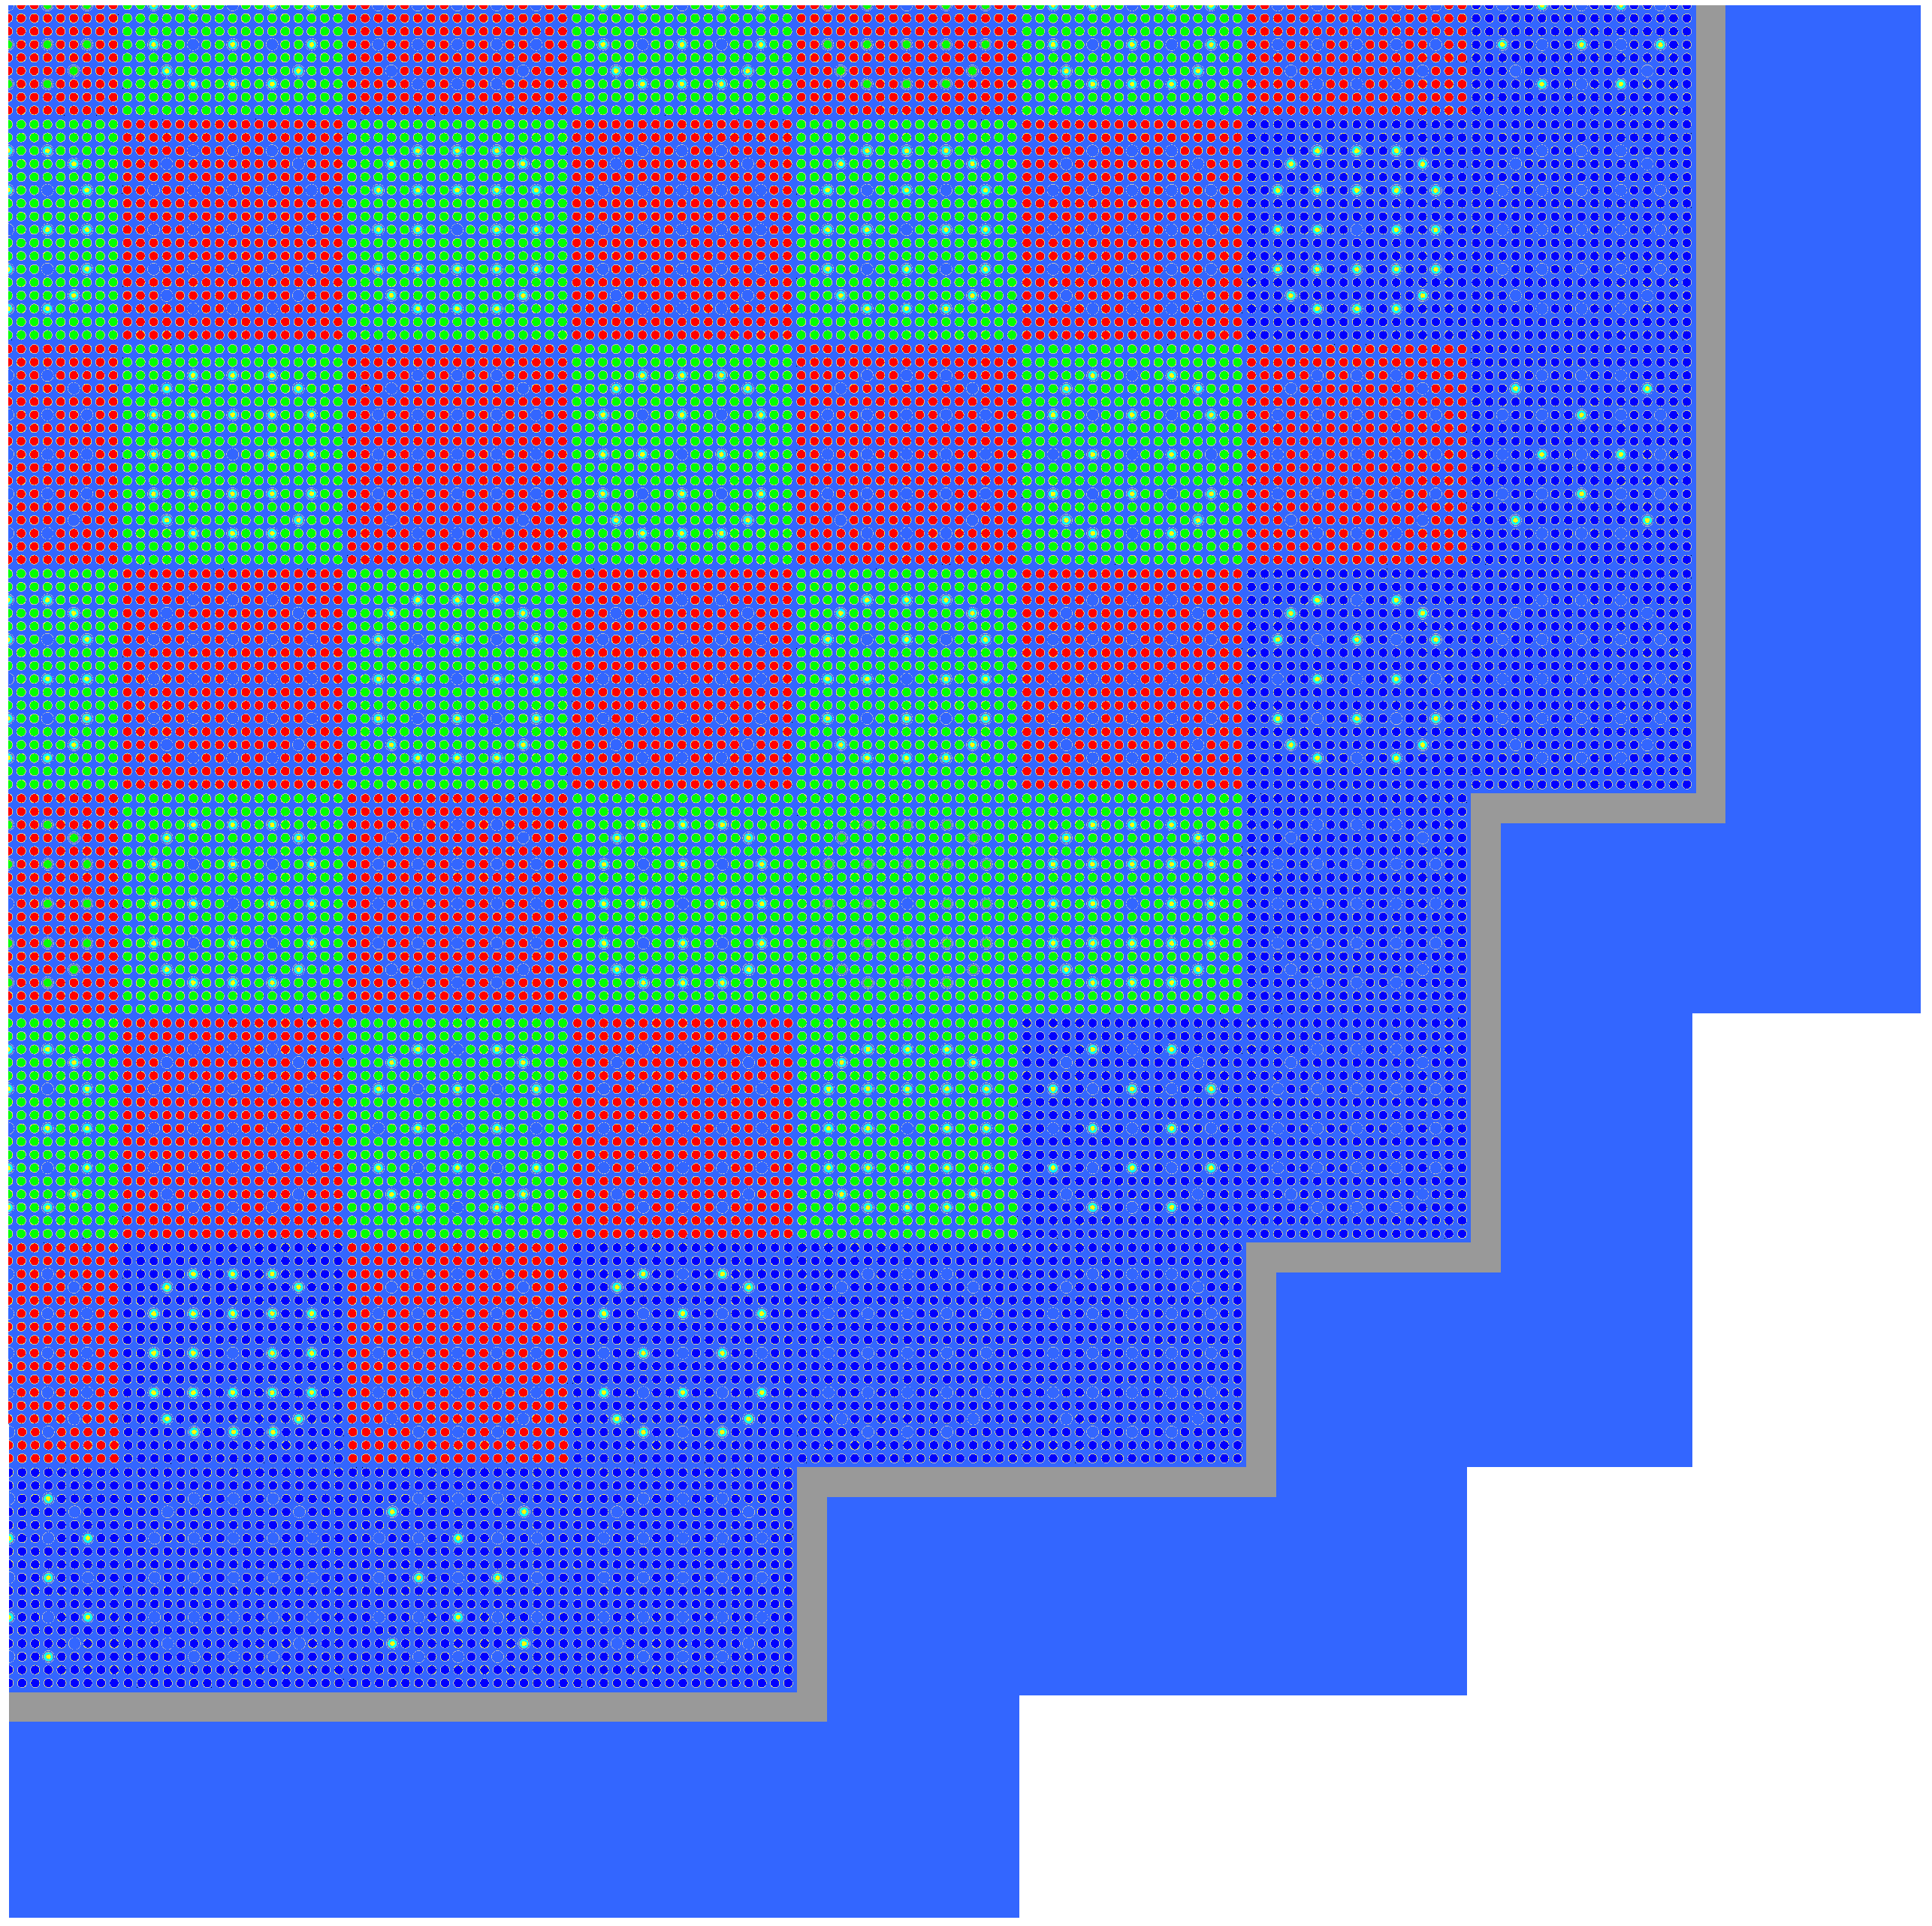
\includegraphics[width=0.48\textwidth]{p5_2D_baffle.png}
\hfill
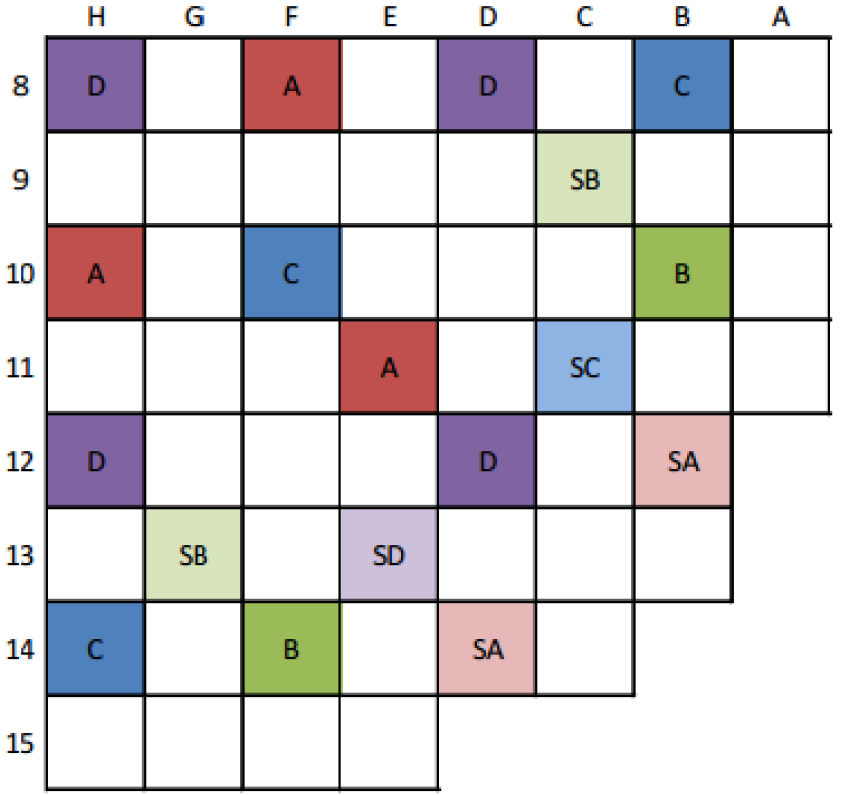
\includegraphics[width=0.48\textwidth]{WB1-cycle1-rodbank-layout.png}
\caption{VERA Problem 5 radial geometry (left) and rod bank positions (right)}\label{f:p5radial}
\end{figure}

\begin{table}
\centering
\caption[VERA Problem 5 Decusping Results]{VERA Problem 5 decusping results for the partially rodded plane}\label{t:p5decusp}
\resizebox{\textwidth}{!}{
  \begin{tabular}{|c|c|c|c|c|c|c|}\hline
    \multirow{2}{*}{Case} & k-eff & \multicolumn{2}{|c|}{Pin Power Differences} & \multicolumn{2}{|c|}{Iterations} & Runtime\\\cline{3-6}
    & Difference (pcm) & RMS & Max & 2D/1D & CMFD & (Core-Hours) \\\hline
    Reference        &  -- & --     & --      & 13 & 481 & 361.7 \\\hline
    No Treatment     & -22 & 6.90\% & 30.55\% & 13 & 523 & 410.7 \\\hline
    Polynomial       &  -5 & 1.15\% &  4.85\% & 13 & 463 & 373.7 \\\hline
    Subplane         &  -5 & 2.09\% & 10.20\% & 13 & 499 & 399.0 \\\hline
    Subplane + CP    &  -1 & 0.50\% &  2.74\% & 13 & 529 & 425.6 \\\hline
  \end{tabular}
}
\end{table}

As with Problem 4, we see that the CP results are the best, with less than 3\% maximum error in the roded plane.  The maximum errors occur in the partially rodded assembly, as expected.  The sub-plane decusping without the CP treatment is worse than in Problem 4, showing the importance of correctly treating the radial effects.  The runtime increase is also between 15\% and 20\% for the sub-plane and CP decusping methods.  Some of this is due to parallel imbalance in the CMFD systems as discussed in Problem 4, but some is also due to the increase in CMFD iterations when using these methods.  Overall, the new methods perform well.  However, nearly 3\% error is still higher than desired when using the 2D/1D method, so there is still room for improvement.

\section{C5G7 Results}

This section will focus on the results for the C5G7 benchmark problems for the subray method of characteristics.  First, 1D results generated by a simple prototype code will be presented, followed by 2D and 3D results from the 2D/1D code MPACT.  While the focus of this section is on subray MOC, the 2D and 3D results will also include the polynomial and subplane collision probabilities decusping techniques to show the accuracy of subray MOC compared with the other methods discussed already.

\subsection{1D Subray}

\begin{figure}[h]
    \centering
    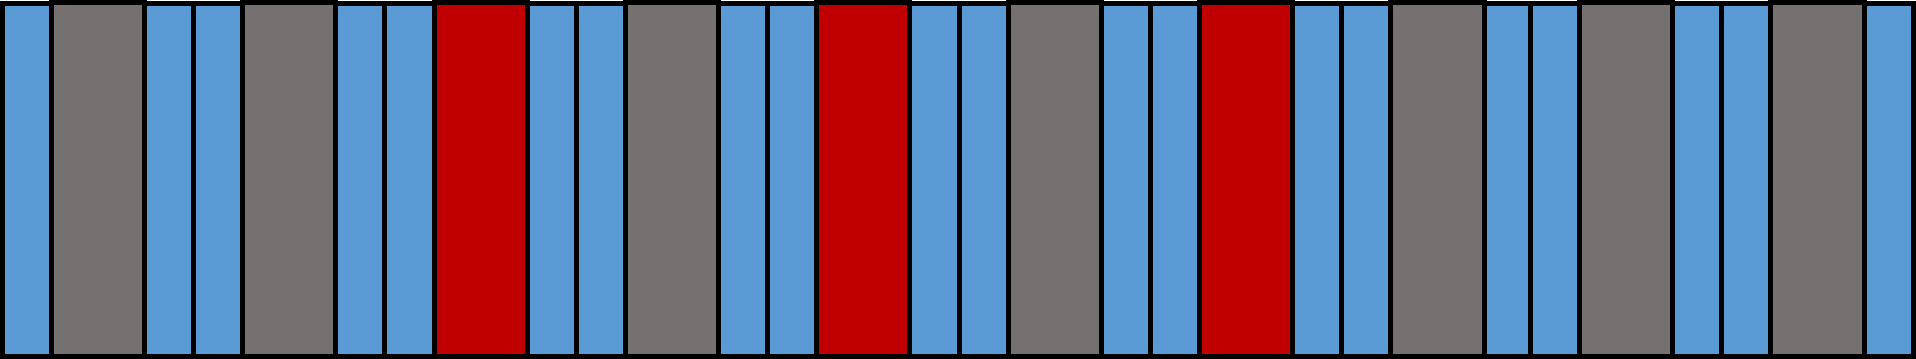
\includegraphics[width=\textwidth]{10pin-slab-geometry.png}
    \caption[Illustration of 1D MOC 10 Pin Geometry]{Illustration of 1D MOC 10 pin test geometry with materials fuel (grey), control rod/moderator mixture (red), and moderator (blue).}\label{f:10pin-geom}
\end{figure}

The 1D subray MOC results were generated using the code described in section \hl{number}.  To show the effectiveness of subray MOC a small 10 pin problem, illustrated in Figure \ref{f:10pin-geom}, was used.  This smaller problem was used because the rods are closer together, making it more difficult to accurately resolve the rods, and to minimize runtime.  To show the effectiveness of the subray method, a series of eigenvalue calculates was performed with the control rod volume fraction varying from 100\% to 0\% to simulate a rod withdrawal.  This was done using traditional MOC and subray MOC to show the correction achieved by using subray MOC.  The reference solution for these calculations is generated by using the volume fractions to mix the fully rodded and unrodded solutions at each iteration and calculating the updated eigenvalue.  The results of these calculations are shown in Figure \ref{f:1d-subray-keff}.

\begin{figure}[h]
    \centering
    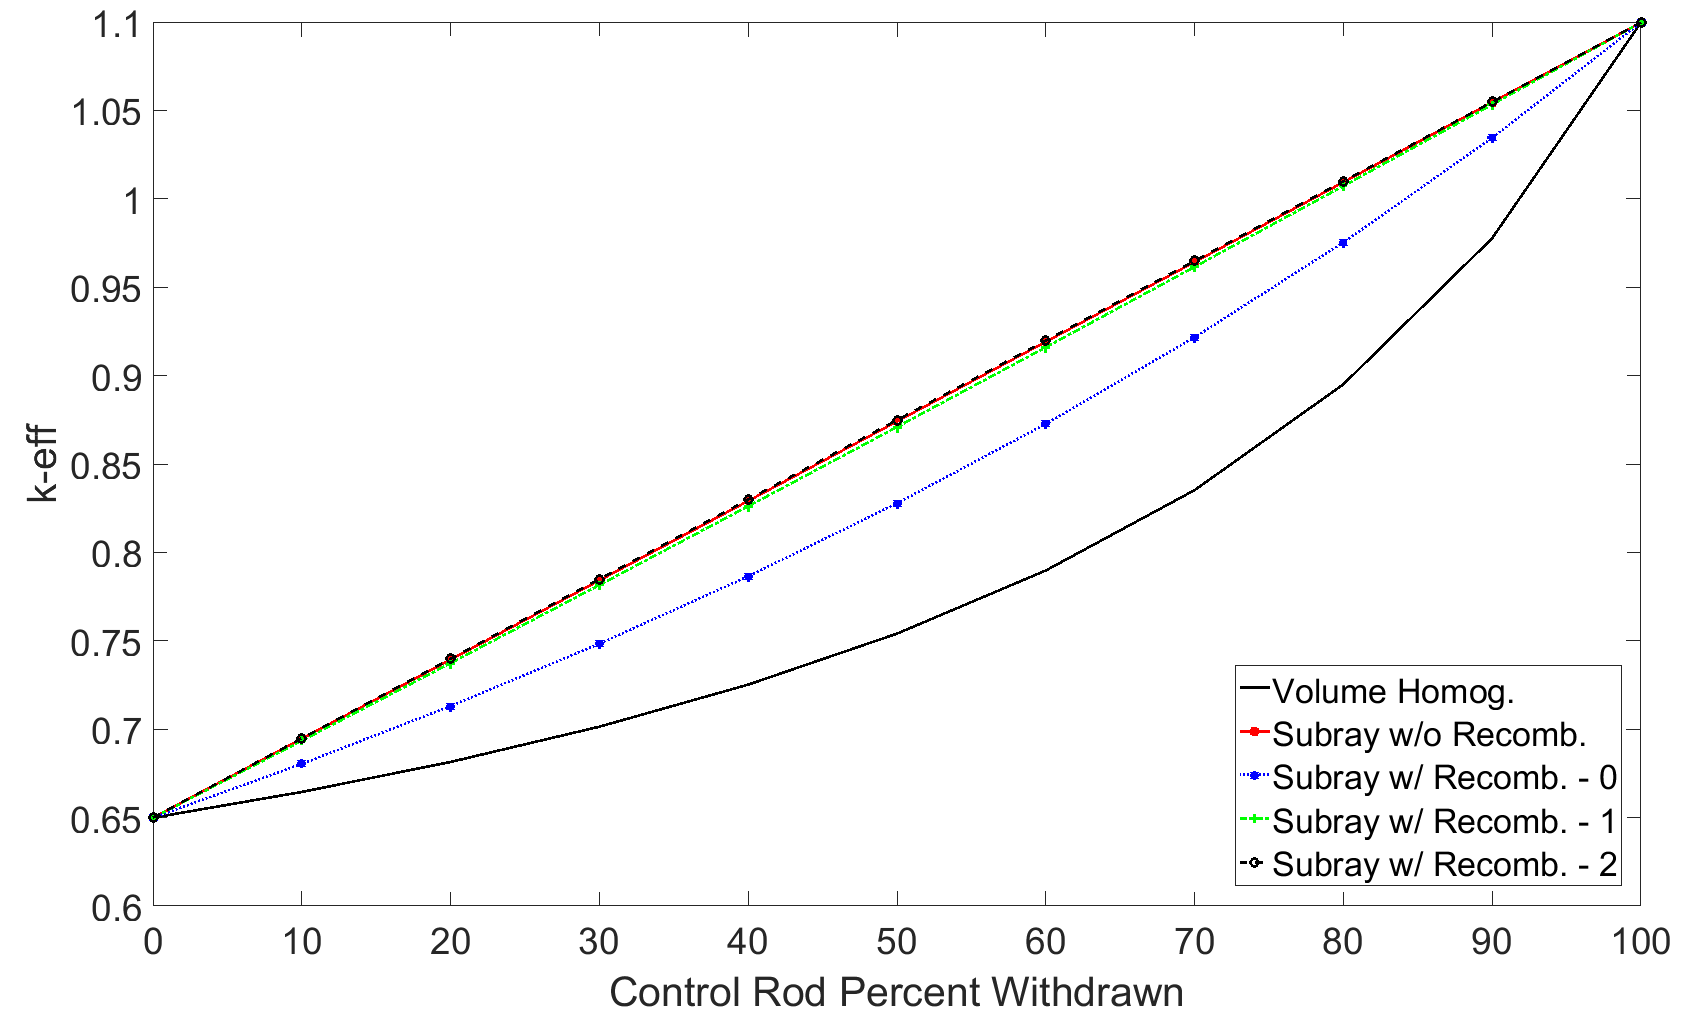
\includegraphics[width=0.8\textwidth]{keff_subray.png}
    \caption{Eigenvalue comparisons for 1D rod withdrawal}\label{f:1d-subray-keff}
\end{figure}

In Figure \ref{f:1d-subray-keff}, the red line is subray without recombination, meaning that two completely separate solves were done each iteration and the resulting scalar fluxes were mixed using volume fractions.  The rodded and unrodded solves have separate angular flux boundary conditions which are saved for each subsequent iteration.  This provides the reference solution.  The volume homogenization solution is a traditional MOC calculation without treating the partially inserted rod.  As is evident, the errors from this method are large, nearing 15\% around 50-60\% withdrawal.  Using subray MOC in only the partially rodded pin cells, indicated in the figure by ``Subray w/ Recomb. - 0'', corrects a significant amount of the error and brings the maximum difference closer to 5\%.  Using a recombination factor of 1 means that subray is now used in all the pin cells between the control rods, correctly resolving the interference effects of the rods and eliminating almost all of the remaining error.  Finally, a recombination factor of 2 extends the subrays all the way to the problem boundary, effectively performing the same calculation as the reference solution.

\begin{figure}[h]
    \centering
    \subfigure[Group 1]{
        \centering
        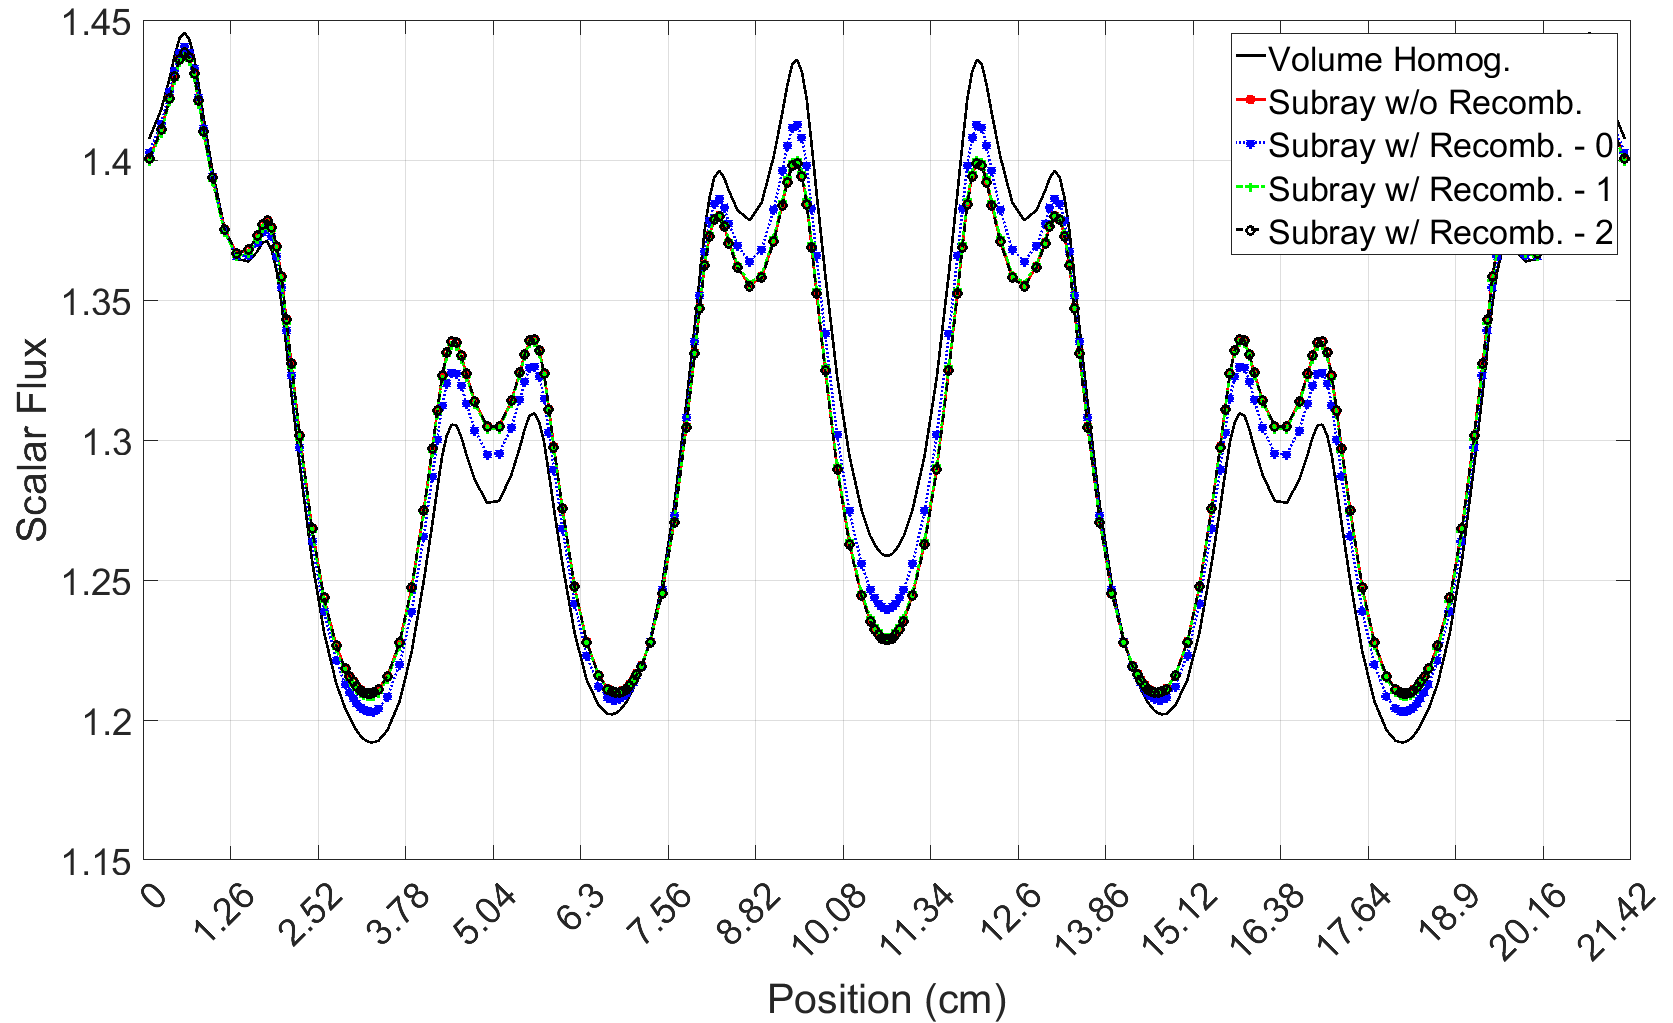
\includegraphics[width=\textwidth]{scalflux1.png}
    }
    ~
    \subfigure[Group 7]{
        \centering
        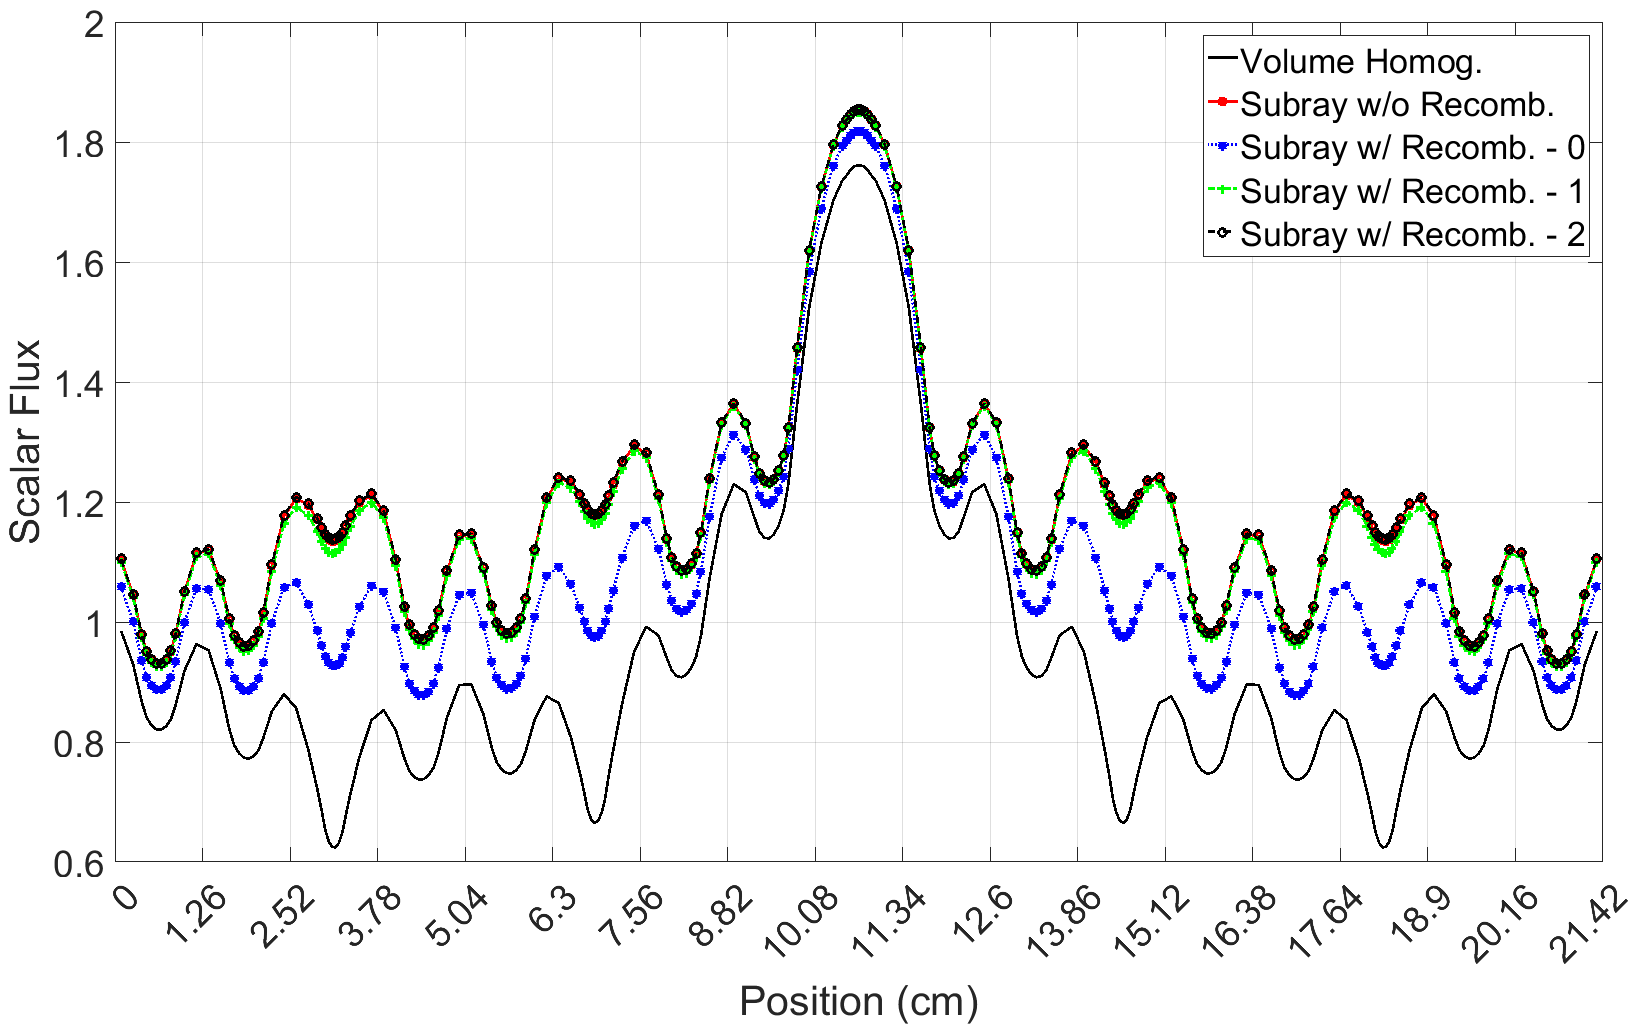
\includegraphics[width=\textwidth]{scalflux7.png}
    }
    \caption{Scalar flux distributions for 1D subray MOC calculations}\label{f:1d-subray-scalflux}
\end{figure}

In addition to the eigenvalue calculations, the scalar flux differences are shown for groups 1 and 7 at 50\% rod withdrawal in Figure \ref{f:1d-subray-scalflux}.  For both groups, it is evident that subray MOC effectively reduces the error caused by the partially inserted rod.  Only performing subray MOC in the rodded pin cells eliminates the majority of the error, but for both the eigenvalue and scalar flux distributions, it is necessary to delay recombination of the angular fluxes for at least one neighboring pin cell to capture the effects of the rod on the source in neighboring pin cells.  This effect is exaggerated by the 1D geometry since the solve is being performed exlusively in the direction that minimizes the distance between pins.  Furthermore, most PWR geometries have at least 2 pins between control rodlets, which further diminishes the effects of rod interference.  While these 1D results do not definitively indicate that recombination should be extended beyond the edge of the partially rodded pin cell, it is important to keep this in mind in the 2D and 3D calculations.

\subsection{2D C5G7}

\subsubsection{UO\texorpdfstring{$_2$}{2} Assembly}

\begin{table}
    \centering
    \caption{2D C5G7 Eigenvalue and Pin Power Differences}\label{t:c5g7-2d-asy-methods}
    \resizebox{\textwidth}{!}{
        \begin{tabular}{l c c l l c l l c l l c l l}
        \toprule
        Rod & Reference & \multicolumn{3}{c}{None} & \multicolumn{3}{c}{Subplane} & \multicolumn{3}{c}{Subplane + CP} & \multicolumn{3}{c}{Subray-0} \\
        Position & k-eff & k-eff & \multicolumn{2}{c}{Pin Powers} & k-eff & \multicolumn{2}{c}{Pin Powers} & k-eff & \multicolumn{2}{c}{Pin Powers} & k-eff & \multicolumn{2}{c}{Pin Powers} \\
        &  &  & RMS & Max &  & RMS & Max &  & RMS & Max &  & RMS & Max \\
        \midrule
        1 &  &  &  &  &  &  &  &  &  &  &  &  &  \\
        2 &  &  &  &  &  &  &  &  &  &  &  &  &  \\
        3 &  &  &  &  &  &  &  &  &  &  &  &  &  \\
        4 &  &  &  &  &  &  &  &  &  &  &  &  &  \\
        5 &  &  &  &  &  &  &  &  &  &  &  &  &  \\
        6 &  &  &  &  &  &  &  &  &  &  &  &  &  \\
        7 &  &  &  &  &  &  &  &  &  &  &  &  &  \\
        8 &  &  &  &  &  &  &  &  &  &  &  &  &  \\
        9 &  &  &  &  &  &  &  &  &  &  &  &  &  \\
        \midrule
        Average &  &  &  &  &  &  &  &  &  &  &  &  &  \\
        \bottomrule
    \end{tabular}
    }
\end{table}

\begin{table}
\centering
\caption{2D C5G7 Eigenvalue and Pin Power Differences}\label{t:c5g7-2d-asy-recomb}
\resizebox{\textwidth}{!}{
    \begin{tabular}{l c c l l c l l c l l c l l}
    \toprule
    Rod & Reference & \multicolumn{3}{c}{Subray-0} & \multicolumn{3}{c}{Subray-1} & \multicolumn{3}{c}{Subray-2} & \multicolumn{3}{c}{Subray-3} \\
    Position & k-eff & k-eff & \multicolumn{2}{c}{Pin Powers} & k-eff & \multicolumn{2}{c}{Pin Powers} & k-eff & \multicolumn{2}{c}{Pin Powers} & k-eff & \multicolumn{2}{c}{Pin Powers} \\
    &  &  & RMS & Max &  & RMS & Max &  & RMS & Max &  & RMS & Max \\
    \midrule
    1 &  &  &  &  &  &  &  &  &  &  &  &  &  \\
    2 &  &  &  &  &  &  &  &  &  &  &  &  &  \\
    3 &  &  &  &  &  &  &  &  &  &  &  &  &  \\
    4 &  &  &  &  &  &  &  &  &  &  &  &  &  \\
    5 &  &  &  &  &  &  &  &  &  &  &  &  &  \\
    6 &  &  &  &  &  &  &  &  &  &  &  &  &  \\
    7 &  &  &  &  &  &  &  &  &  &  &  &  &  \\
    8 &  &  &  &  &  &  &  &  &  &  &  &  &  \\
    9 &  &  &  &  &  &  &  &  &  &  &  &  &  \\
    \midrule
    Average &  &  &  &  &  &  &  &  &  &  &  &  &  \\
    \bottomrule
    \end{tabular}
}
\end{table}

\subsubsection{2D Core -- Rodded Center Assembly}

\begin{table}
    \centering
    \caption{2D C5G7 Eigenvalue and Pin Power Differences}\label{t:c5g7-2d-center-methods}
    \resizebox{\textwidth}{!}{
        \begin{tabular}{l c c l l c l l c l l c l l}
            \toprule
            Rod & Reference & \multicolumn{3}{c}{None} & \multicolumn{3}{c}{Subplane} & \multicolumn{3}{c}{Subplane + CP} & \multicolumn{3}{c}{Subray-0} \\
            Position & k-eff & k-eff & \multicolumn{2}{c}{Pin Powers} & k-eff & \multicolumn{2}{c}{Pin Powers} & k-eff & \multicolumn{2}{c}{Pin Powers} & k-eff & \multicolumn{2}{c}{Pin Powers} \\
            &  &  & RMS & Max &  & RMS & Max &  & RMS & Max &  & RMS & Max \\
            \midrule
            1 &  &  &  &  &  &  &  &  &  &  &  &  &  \\
            2 &  &  &  &  &  &  &  &  &  &  &  &  &  \\
            3 &  &  &  &  &  &  &  &  &  &  &  &  &  \\
            4 &  &  &  &  &  &  &  &  &  &  &  &  &  \\
            5 &  &  &  &  &  &  &  &  &  &  &  &  &  \\
            6 &  &  &  &  &  &  &  &  &  &  &  &  &  \\
            7 &  &  &  &  &  &  &  &  &  &  &  &  &  \\
            8 &  &  &  &  &  &  &  &  &  &  &  &  &  \\
            9 &  &  &  &  &  &  &  &  &  &  &  &  &  \\
            \midrule
            Average &  &  &  &  &  &  &  &  &  &  &  &  &  \\
            \bottomrule
        \end{tabular}
    }
\end{table}

\begin{table}
    \centering
    \caption{2D C5G7 Eigenvalue and Pin Power Differences}\label{t:c5g7-2d-center-recomb}
    \resizebox{\textwidth}{!}{
        \begin{tabular}{l c c l l c l l c l l c l l}
            \toprule
            Rod & Reference & \multicolumn{3}{c}{Subray-0} & \multicolumn{3}{c}{Subray-1} & \multicolumn{3}{c}{Subray-2} & \multicolumn{3}{c}{Subray-3} \\
            Position & k-eff & k-eff & \multicolumn{2}{c}{Pin Powers} & k-eff & \multicolumn{2}{c}{Pin Powers} & k-eff & \multicolumn{2}{c}{Pin Powers} & k-eff & \multicolumn{2}{c}{Pin Powers} \\
            &  &  & RMS & Max &  & RMS & Max &  & RMS & Max &  & RMS & Max \\
            \midrule
            1 &  &  &  &  &  &  &  &  &  &  &  &  &  \\
            2 &  &  &  &  &  &  &  &  &  &  &  &  &  \\
            3 &  &  &  &  &  &  &  &  &  &  &  &  &  \\
            4 &  &  &  &  &  &  &  &  &  &  &  &  &  \\
            5 &  &  &  &  &  &  &  &  &  &  &  &  &  \\
            6 &  &  &  &  &  &  &  &  &  &  &  &  &  \\
            7 &  &  &  &  &  &  &  &  &  &  &  &  &  \\
            8 &  &  &  &  &  &  &  &  &  &  &  &  &  \\
            9 &  &  &  &  &  &  &  &  &  &  &  &  &  \\
            \midrule
            Average &  &  &  &  &  &  &  &  &  &  &  &  &  \\
            \bottomrule
        \end{tabular}
    }
\end{table}

\subsubsection{2D Core -- Rodded Corner Assembly}

\begin{table}
    \centering
    \caption{2D C5G7 Eigenvalue and Pin Power Differences}\label{t:c5g7-2d-corner-methods}
    \resizebox{\textwidth}{!}{
        \begin{tabular}{l c c l l c l l c l l c l l}
            \toprule
            Rod & Reference & \multicolumn{3}{c}{None} & \multicolumn{3}{c}{Subplane} & \multicolumn{3}{c}{Subplane + CP} & \multicolumn{3}{c}{Subray-0} \\
            Position & k-eff & k-eff & \multicolumn{2}{c}{Pin Powers} & k-eff & \multicolumn{2}{c}{Pin Powers} & k-eff & \multicolumn{2}{c}{Pin Powers} & k-eff & \multicolumn{2}{c}{Pin Powers} \\
            &  &  & RMS & Max &  & RMS & Max &  & RMS & Max &  & RMS & Max \\
            \midrule
            1 &  &  &  &  &  &  &  &  &  &  &  &  &  \\
            2 &  &  &  &  &  &  &  &  &  &  &  &  &  \\
            3 &  &  &  &  &  &  &  &  &  &  &  &  &  \\
            4 &  &  &  &  &  &  &  &  &  &  &  &  &  \\
            5 &  &  &  &  &  &  &  &  &  &  &  &  &  \\
            6 &  &  &  &  &  &  &  &  &  &  &  &  &  \\
            7 &  &  &  &  &  &  &  &  &  &  &  &  &  \\
            8 &  &  &  &  &  &  &  &  &  &  &  &  &  \\
            9 &  &  &  &  &  &  &  &  &  &  &  &  &  \\
            \midrule
            Average &  &  &  &  &  &  &  &  &  &  &  &  &  \\
            \bottomrule
        \end{tabular}
    }
\end{table}

\begin{table}
    \centering
    \caption{2D C5G7 Eigenvalue and Pin Power Differences}\label{t:c5g7-2d-corner-recomb}
    \resizebox{\textwidth}{!}{
        \begin{tabular}{l c c l l c l l c l l c l l}
            \toprule
            Rod & Reference & \multicolumn{3}{c}{Subray-0} & \multicolumn{3}{c}{Subray-1} & \multicolumn{3}{c}{Subray-2} & \multicolumn{3}{c}{Subray-3} \\
            Position & k-eff & k-eff & \multicolumn{2}{c}{Pin Powers} & k-eff & \multicolumn{2}{c}{Pin Powers} & k-eff & \multicolumn{2}{c}{Pin Powers} & k-eff & \multicolumn{2}{c}{Pin Powers} \\
            &  &  & RMS & Max &  & RMS & Max &  & RMS & Max &  & RMS & Max \\
            \midrule
            1 &  &  &  &  &  &  &  &  &  &  &  &  &  \\
            2 &  &  &  &  &  &  &  &  &  &  &  &  &  \\
            3 &  &  &  &  &  &  &  &  &  &  &  &  &  \\
            4 &  &  &  &  &  &  &  &  &  &  &  &  &  \\
            5 &  &  &  &  &  &  &  &  &  &  &  &  &  \\
            6 &  &  &  &  &  &  &  &  &  &  &  &  &  \\
            7 &  &  &  &  &  &  &  &  &  &  &  &  &  \\
            8 &  &  &  &  &  &  &  &  &  &  &  &  &  \\
            9 &  &  &  &  &  &  &  &  &  &  &  &  &  \\
            \midrule
            Average &  &  &  &  &  &  &  &  &  &  &  &  &  \\
            \bottomrule
        \end{tabular}
    }
\end{table}

\subsection{3D C5G7}